% Diese Zeile bitte -nicht- aendern.
\documentclass[course=erap]{aspdoc}

%%%%%%%%%%%%%%%%%%%%%%%%%%%%%%%%%
%% TODO: Ersetzen Sie in den folgenden Zeilen die entsprechenden -Texte-
%% mit den richtigen Werten.
\newcommand{\theGroup}{105} % Beispiel: 42
\newcommand{\theNumber}{A326} % Beispiel: A123
\author{Benedikt Falk \and Fabian Strobl \and Severin Leitner}
\date{Sommersemester 2023} % Beispiel: Wintersemester 2019/20
%%%%%%%%%%%%%%%%%%%%%%%%%%%%%%%%%

% Diese Zeile bitte -nicht- aendern.
\title{Gruppe \theGroup{} -- Abgabe zu Aufgabe \theNumber}
\usepackage{url}
\begin{document}
    \maketitle

    \section{Einleitung}

    Es gibt viele Möglichkeiten \begin{math}\sqrt{2}\end{math} beliebig genau zu berechnen. In unserem Projekt wurde dies mithilfe der Exponentiation der Matrix \begin{align}
                                                                                                                                                                     \begin{pmatrix}
                                                                                                                                                                         0 & 1\\
                                                                                                                                                                         1 & 2
                                                                                                                                                                     \end{pmatrix}
    \end{align}
    realisiert. Durch das n-fache Multiplizieren dieser Matrix mit sich selbst erhält man schlussendlich die Matrix
    \begin{align}
        \begin{pmatrix}
            x_{n-1} & x_n \\
            x_n  & x_{n+1}
        \end{pmatrix}. \end{align}  Die Konstante \begin{math} \sqrt{2} \end{math} erhält man nun durch die Rechenvorschrift
    \begin{align}
        \lim\limits_{n \to \infty} 1 + \frac{x_n}{x_{n+1}} = \sqrt{2}.
    \end{align}
    Wieso das funktioniert, wird im Kapitel \glqq Korrektheit \grqq\space kurz erklärt ~\ref{Korrektheit}. Das Verfahren hat viele Anwendungsbereiche. Zu diesen gehört beispielsweise auch Pagerank, der Algorithmus, den Google für sehr lange Zeit genutzt hat, um Suchergebnisse zu sortieren.~\cite{pagerank} Ebenso benutzten Markov-Ketten dieses Verfahren. Bei den Ketten handelt es sich um einen stochastischen Prozess, welcher auch für die Informatik von hoher Bedeutung ist.
    In unserer Implementierung bestand die Schwierigkeit darin, das Ergebnis auch dann richtig auszugeben, wenn \begin{math}
                                                                                                                    x_n
    \end{math} die Speichergröße der herkömmlichen Datentypen überschreitet. Unsere Aufgabe war es nun, \begin{math}
                                                                                                            \sqrt{2}
    \end{math} auf beliebig viele Binärstellen auszugeben. Da es sich bei \begin{math}
                                                                              \sqrt{2}
    \end{math} um eine irrationale Zahl handelt, können theoretisch unendlich viele binäre Nachkommastellen ausgegeben werden. Es wird vermutet, dass es sich hierbei sogar um die erste Zahl handelt, welche als irrational identifiziert wurde.\cite{first} Erst letztes Jahr wurde ein neuer Genauigkeitsrekord aufgestellt, als Tizian Hanselmann \begin{math}
                                                                                                                                                                                                                                                                                                                                                          \sqrt{2}
    \end{math} auf 10 000 000 001 000 (10 Billiarden und 1000) Stellen berechnete.~\cite{record} Um die Berechnung durchzuführen und den \glqq Trade-Off \grqq zwischen  Genauigkeit ~\ref{Genauigkeit}, Korrektheit ~\ref{Korrektheit} und Geschwindigkeit ~\ref{Performance} zeigen zu können, haben wir unterschiedliche Algorithmen und Datenstrukturen genutzt. Wir haben u.a. zwei Structs implementiert, die nur durch den Speicherplatz begrenzt, beliebig große Zahlen speichern können, sowie eine Datenstruktur, die Zahlen als Fixkommazahlen betrachtet und entsprechend ein Komma setzt.

    \newpage
    \section{Lösungsansatz}
    \subsection{BigNum Struct}
    Es hat sich sehr schnell gezeigt, dass die normalen Datenstrukturen, die in C gegeben sind, nicht ausreichen, um genügend große Zahlen zu speichern. Bereits bei der sechsten Quadrierung der Matrix ist die Zahl so groß, dass 64 Bit nicht mehr ausreichen, um diese Zahl darzustellen. Deswegen haben wir uns dazu entschieden, eine eigene Datenstruktur zu implementieren, die Zahlen beliebiger Größe speichert. Als erstes haben wir diese Struktur angelehnt an eine Fix-Komma-Struktur aufgebaut. Dies bedeutet, dass wir ein Struct erstellt haben, welches eine vordefinierte Menge an Long-Arrays implementiert. Ebenso war in dem Struct \glqq BigNum\grqq eine Konstante für die Stelle, an der das Komma stehen soll, reserviert. Zusätzlich war zur Berechnung ebenso die Länge (also die Anzahl der Arrays in diesem Struct) abgespeichert. Nun kann theoretisch jede beliebige Zahl intern repräsentiert und dargestellt werden. Die einzige Begrenzung wird durch den Hardwarespeicher festgelegt.
    Bei der Implementierung der Grundrechenarten auf diesem Struct hat sich aber herausgestellt, dass man beispielsweise die Multiplikation mit Ganzzahlen deutlich schneller und effizienter durchführen kann, als mit Fixkommazahlen, weil der Teil zur Verschiebung der Kommastelle entfällt. Aus diesem Grund haben wir eine ähnliche Datenstruktur entwickelt, welche auf ein Komma verzichtet. Das Struct besteht aus einer Variablen für die Länge der abgespeicherten Zahl, sowie einem long long Pointer, die wie folgt Anwendung finden. Die Zahlen werden in den einzelnen Teilen des long Arrays gespeichert, wobei die kleinste Zahl, also die Einser-, Zehner-Stellen usw. an der 0. Stelle im Array gespeichert werden. Die Variable für die Länge speichert die Anzahl der Arrays ab, die für die Darstellung der Zahl benötigt werden. In jedem Array werden Zahlen zwischen 0 und 999.999.999 gespeichert.
    Auch wenn in jedem Array Zahlen bis \begin{math}
                                            2^{64}
    \end{math} gespeichert werden könnten, haben wir uns auf diesen Bereich begrenzt, um einen Overflow bei der Multiplikation zu verhindern. Da length nun aber nur die Anzahl der Arrays beschreibt und wir auch wissen möchten, wieviele Stellen die gespeicherte Zahl hat, betrachten wir nur die Arrays, in denen keine führenden Nullen stehen und multiplizieren diese Zahl mit 9 - für 9 Stellen in jedem Array - und subtrahieren die übrigen Nullen aus der Speicherzelle, die die führenden Stellen beinhaltet. Im Weiteren werden die Grundrechenarten auf dem neu definierten Struct näher beschrieben.
    \subsubsection{Addition}
    Für die Addition werden zwei Arrays, der übergebenen BigNum Pointer, paarweise addiert und die Summe modulo 1 Milliarden an die entsprechende Stelle im Ergebnis gespeichert. Außerdem wird eine Variable $carry$ initialisiert, die 1 ist, wenn das Ergebnis der Addition $\geq$ 1 Milliarden war, sonst 0. Das Carry wird dann für die Berechnung der nächsten Stelle verwendet. Wenn ein Summand mehr Stellen hat als der andere, wird einfach der größere Summand übernommen. Das Ergebnis hat maximal die Länge der längeren Zahl +1;
    \subsubsection{Subtraktion}
    Der Methode werden zwei BigNum Pointer als Parameter übergeben. Für die Subtraktion gehen wir davon aus, dass der erste Subtrahend  mindestens so viele Stellen hat wie der Zweite, da in unserere Implementierung keine negativen Zahlen vorkommen. Nun wird der zweite Subtrahend arrayweise von dem ersten abgezogen und auf das Ergebnis addiert. Sollte der Wert kleiner als 0 sein, so wird 1 Milliarden an dieser Stelle im Array addiert und von der nächsthöheren Stelle 1 abgezogen. Sollte der erste Subtrahend mehr Stellen als der Zweite haben, werden die restlichen Zahlen nur noch auf das Ergebnis an die entsprechenden Stellen geschrieben (entspricht -0). Das Ergebnis hat maximal so viele Stellen, wie die erste Zahl.
    \subsubsection{Multiplikation}
    Der Multiplikation werden zwei BigNum Pointer übergeben und durch eine For-Schleife über eine der beiden Zahlen wird das Produkt berechnet. In jeder Iteration wird der andere Faktor traversiert und jeder Eintrag mit dem der jeweiligen Stelle im ersten Faktor multipliziert und das Ergebnis modulo 1 Milliarden an der richtigen Stelle im Ergebnis gespeichert. Sollte es dabei zu einem Übertrag kommen, wird er zum Eintrag des Ergebnisses am nächst höheren Index addiert. Das Ergebnis hat maximal so viele Stellen, wie die Summe der Längen beider Faktoren.
    \subsubsection{Compare}
    Die Compare Methode wird für die nachfolgende Divison benötigt. Sie nimmt zwei Pointer auf Bignums und vergleicht diese miteinander. Wenn die eine Zahl länger als die andere ist, ist kein weiterer Vergleich nötig, da es keine negativen Zahlen geben kann. In diesem Fall wird 1, bzw. -1 zurückgegeben. Liefert diese Methode noch kein Ergebnis, werden die Zahlen, beginnend bei der \glqq most significant number\grqq, arrayweise verglichen. Sobald eine Zahl in einem Array größer ist als die andere, wird das entsprechende Ergebnis zurückgegeben. Sollten die beiden Zahlen gleich groß sein wird 0 zurückgegeben.
    \subsubsection{Division}
    Die Divison bekommt zwei BigNum Pointer und einen long long Wert, der die Anzahl der Nachkommastellen, die berechnet werden sollen, beinhaltet und gibt einen Char Pointer der Länge der gewünschten Genauigkeit zurück. Das ist möglich, da die Division stets nur am Ende der Berechnungen aufgerufen wird und das Array dann zur Ausgabe des Ergebnisses auf der Konsole genutzt wird. In der Methode wird jede Stelle des Ergebnisses einzeln berechnet, indem man vergleicht, ob number1 $\geq$ number2 gilt. Sollte das der Fall sein, zieht man so oft die erste Zahl von der zweiten ab, bis number1 < number2 ist. Die Anzahl der durchgeführten Subtraktionen entspricht dann einer Ziffer im Ergebnis. Sobald number1 < number2 wird number1 mit 10 multipliziert und der Prozess beginnt von vorne. Sollte nach der Multiplikation number1 < number2 gelten, so war die Ziffer eine 0 und es wird erneut mit 10 multipliziert. Sollten die Zahlen zu einem Zeitpunkt 0 werden, so ist bereits die maximale Genauigkeit berechnet und die Methode stellt sicher, dass der String nullterminiert ist und gibt den Char Pointer zurück.
    \subsubsection{Hexadezimal}
    Die Umwandlung einer Zahl vom Dezimalsystem ins Hexadezimalsystem hat sich schwerer, als ursprünglich erwartet, herausgestellt, da die bereits existierenden Funktionen zur Umwandlung eine bestimmte Obergrenze für die Zahlengröße besitzen, wie die Größe eines Integer oder eines unsigned long longs. In unserer Implementierung soll diese Funktion jedoch Zahlen mit beliebiger Größe umwandeln können.
    Die Funktion berechnet mod 16 der Zahl, die der String, repräsentiert und schreibt das Ergebnis in Hexadezimal Schreibweise in einen Ergebnis String. Danach wird der Int String durch 16 geteilt und von vorne begonnen.
    Dieses Verfahren wird so lange wiederholt, bis der Int String nur noch 0 enthält, woraufhin der Ergebnis String reversed wird und die führenden Nullen entfernt werden.
    Die Laufzeitklasse dieser Funktion befindet sich in \begin{math}\mathcal{O}(
    n^2
    \end{math})
    mit n = Anzahl der Ziffern.
    \subsection{Schnelle Exponentiation}\label{Schnelle Exponentiation}
    Als ersten zusätzlichen Schritt zur Performanceverbesserung haben wir dann die schnelle Exponentiation implementiert. Diese funktioniert für integer Zahlen wie folgt: Für eine Zahl x, welche man n mal exponieren möchte (also \begin{math}
                                                                                                                                                                                                                                         x^n
    \end{math}), findet man zuerst die kleinste Zahl z, für die \begin{math}
                                                                    2^z > n
    \end{math} gilt. Dann entspricht (z-1) der Anzahl der erforderlichen Quadrierungen. Zusätzlich zerlegt man den Exponent n in seine Binärdarstellung und liest die Stellen ab, an denen das Bit gesetzt ist.
    Man multipliziert dann das Ergebnis immer mit der i-ten Quadrierung, wenn an der i-ten Stelle in \begin{math} x_2 \end{math} eine eins steht. Diese Methode basiert auf der Beobachtung, dass
    \begin{align}
        x^n = \begin{cases}
                  x(x^2)^{(n-1)/2} &\text{if } n\ is\ odd \\
                  (x^2)^{n/2} &\text{if } n\ is\ even
        \end{cases}
    \end{align}
    gilt. ~\cite{recursion} Dies ist eine rekursiv definierte Funktion, welche man entweder rekursiv oder iterativ implementieren kann. Während die naive Implementierung einer solchen Exponentiation in $\mathcal{O}$ (n) liegt, besitzt die Methode der schnellen Exponentiation eine Laufzeit von  $\mathcal{O}$ (\begin{math}
                                                                                                                                                                                                                                                                                                                          log_2(n)
    \end{math}) .
    \subsubsection{Beispielrechnung Matrix}\label{Beispielrechnung}
    In unserem Fall mussten wir das Verfahren noch auf Matrizen übertragen. Im Prinzip kann man diese Methode jedoch analog auf eine quadratische Matrix, wie unsere, angewendet werden. Zur Veranschaulichung zeigt das folgende Beispiel die schnelle Exponentiation für den Exponenten 11.
    \begin{table}[ht]\label{Quadrierungen}
    \centering
    \begin{tabular}{c| c}
        $i$ & $a_i$ \\
        \hline
        0 & $\begin{pmatrix}
                 0 & 1 \\
                 1 & 2
        \end{pmatrix} = \begin{pmatrix}
                            0 & 1 \\
                            1 & 2
        \end{pmatrix}$ \\
        \hline
        1 & $\begin{pmatrix}
                 0 & 1 \\
                 1 & 2
        \end{pmatrix}^2 = \begin{pmatrix}
                              1 & 2 \\
                              2 & 5
        \end{pmatrix}$ \\
        \hline
        2 & $\begin{pmatrix}
                 1 & 2 \\
                 2 & 5
        \end{pmatrix}^2 = \begin{pmatrix}
                              5 & 12 \\
                              12 & 29
        \end{pmatrix}$ \\
        \hline
        3 & $\begin{pmatrix}
                 5 & 12 \\
                 12 & 29
        \end{pmatrix}^2 = \begin{pmatrix}
                              169 & 408 \\
                              408 & 985
        \end{pmatrix}$ \\

    \end{tabular}
    \caption{Quadrierungen}
    \end{table}
    Tabelle 1 \ref{Quadrierungen}zeigt die vier Quadierungsschritte für die Matrix. Zunächst betrachten wir die Binärdarstellung der Zahl 11 = \begin{math}  1011_b\end{math}. Wir setzen die Matrix \begin{math}
                                                                                                                                                                                                         R =
                                                                                                                                                                                                         E_n = \begin{pmatrix}
                                                                                                                                                                                                                   1 & 0 \\
                                                                                                                                                                                                                   0 & 1 \\
                                                                                                                                                                                                         \end{pmatrix} \end{math}  und \begin{math}
                                                                                                                                                                                                                                           A = \begin{pmatrix}
                                                                                                                                                                                                                                                   0 & 1 \\
                                                                                                                                                                                                                                                   1 & 2 \\
                                                                                                                                                                                                                                           \end{pmatrix}
    \end{math}.  Die nächste 2er Potenz größer der 11 (Exponent) ist die 16, bzw. $2^{4}$, weshalb wir vier Schleifendurchläufe simulieren müssen. Beginnend bei \begin{math}
                                                                                                                                                                     i = 0
    \end{math} führen wir für jeden Iterationsschritt die folgenden beiden Schritte aus: \begin{enumerate}
                                                                                             \item Wenn das ite Bit in der Binärdarstellung gesetzt ist, setzen wir \begin{math}
                                                                                                                                                                        R = RA
                                                                                             \end{math},  wobei \begin{math}
                                                                                                                    RA
                                                                                             \end{math} als die Matrixmultiplikation definiert wird
                                                                                             \item Unabängig von der Binärdarstellung multiplizieren wir \begin{math}
                                                                                                                                                             A
                                                                                             \end{math} in jedem Schritt mit sich selbst (\begin{math}
                                                                                                                                              A = A^2
                                                                                             \end{math})
    \end{enumerate} Das Ergebnis liefert \begin{math}
                                             \begin{pmatrix}
                                                 0 & 1 \\
                                                 1 & 2 \\
                                             \end{pmatrix}^{11} = \begin{pmatrix}
                                                                      2378 & 5741 \\
                                                                      5741 & 13860 \\
                                             \end{pmatrix}
    \end{math} ohne dass wir die Matrix elf mal mit sich selbst multipliziert haben.
    \subsubsection{Korrektheit}\label{Korrektheit}
    Aber wieso führt die oben genannte Rechenvorschrift überhaupt dazu, dass man $\sqrt{2}$ approximieren kann?
    Dies liegt daran, dass eine diagonalisierbare Matrix - wie unsere - mit Exponentiation zu dem Eigenvektor mit dem dominanten Eigenwert konvergiert. In unserem Fall handelt es sich bei dem dominanten Eigenwert um $\lambda_1 = 1+\sqrt{2}$ und der dazugehörige Eigenvektor ist $\begin{pmatrix}
                                                                                                                                                                                                                                                                                           -1 + \sqrt{2} \\
                                                                                                                                                                                                                                                                                           1
    \end{pmatrix}$.
    Hier kann man schnell erkennen, wie nun die in der Einleitung genannte Rechenvorschrift zustande kommt.~\cite{konvergiert} Jedoch müssen wir auch noch korrekt exponieren, deshalb stellt sich die Frage, warum funktioniert die schnelle Exponentation?
    Zur Vereinfachung kehren wir zurück zur ganzzahligen Exponentiation: Betrachten wir im Folgenden \begin{math}
                                                                                                         7^{11}
    \end{math}. Zunächst schreiben wir 11 als
    \begin{align}
        1*2^3 + 1*2^2 + 0*2^1 + 1*2^0
    \end{align} So ergibt sich \begin{math}
                                   7^{2^3 + 2^2+2^0}
    \end{math} bzw. \begin{math}
                        7^{2^3} * 7^{2^2} * 7^{2^0}
    \end{math}. Das Muster lässt sich bereits erkennen. Analog zu den Matrizen beginnen wir mit der \begin{math}
                                                                                                        1
    \end{math} und multiplizieren sie mit \begin{math}
                                              7^{2^0}
    \end{math}.\cite{blatt}
    Anschließend quadrieren wir die Basis und gehen in den nächsten Schritt. Das 2. Bit ist nicht gesetzt, demnach multiplizieren wir die Basis erneut mit sich selbst, ohne das Zwischenergebnis damit zu verechnen. Der Schritt wird für alle Bits in der Binärdarstellung des Exponenten wiederholt. Das Ergebnis liefert \begin{math}
                                                                                                                                                                                                                                                                                                                                 7^{11} = 1977326743
    \end{math}. Das Prinzip lässt sich wie oben gezeigt ~\ref{Beispielrechnung} auf Matrizen übertragen.
    \subsubsection{Annäherung}
    Soweit haben wir nur die Matrix entsprechend oft exponiert, aber welche Schritte fehlen noch bis zum gewünschten Ergebnis \begin{math}
                                                                                                                                  \sqrt{2}
    \end{math} ? Zunächst teilen wir den oberen rechten Eintrag \begin{math}
                                                                    x_n
    \end{math} durch den unteren rechten Eintrag \begin{math}
                                                     x_{n+1}
    \end{math} und addieren 1 zum Ergebnis. WolframAlpha liefert nach elf maligem exponieren \begin{math}
                                                                                                 1.414213564\ldots
    \end{math} und somit die Quadratwurzel von 2 auf 8 Nachkommastellen genau. Für genauere Ergebnisse muss die Matrix öfter exponiert werden. Da sich die Stellen der Zahlen exponentiell vervielfachen, zeigen sich erste Performanceschwierigkeiten auf, welche bei der Division auftreten. Es gibt unterschiedliche Divisionsverfahren, eines davon ist das Newton-Raphson-Verfahren.
    \subsection{Newton-Raphson-Verfahren}
    Bei dieser Methode wird statt dem Teilen durch Annäherung der Kehrbruch des Nenners berechnet und das Ergebnis durch eine Multiplikation berechnet.
    Ursprünglich ist das Newton-Raphson-Verfahren dazu entwickelt worden, die Wurzel einer Funktion \begin{math}
                                                                                                        f(x) = 0
    \end{math} zu finden. Bei diesem Verfahren handelt es sich um ein Approximationsverfahren, d.h. man versucht iterativ immer genauere Ergebnisse zu finden. Das Verfahren ist das am weitesten verbreitete, um die Annäherung einer Quadratwurzel einer Funktion zu finden. Man beginnt mit einer Abschätzung für den Startwert \begin{math}
                                                                                                                                                                                                                                                                                                                                       x_0
    \end{math}, welche sehr großen Einfluss auf die Korrektheit des Algorithmus hat, und deswegen vorsichtig gewählt werden sollte.~\cite{newtonmethod}
    Nun wollen wir jedoch nicht die Quadratwurzel einer Funktion finden, sondern eine effiziente Division durchführen. Um dies erreichen zu können, muss man den Algorithmus etwas anpassen. Wir wollen das Reziproke einer Zahl finden, um dann das Endergebnis durch Multiplikation mit dem Kehrbruch
    zu berechnen. Als effiziente Formel dafür hat sich
    \begin{align}
        x_{i+1} = x_i * (2- d*x_i)
    \end{align}
    für geeignet erwiesen. Hierbei werden bei jeder Iteration zwei Multiplikationen und eine Subtraktion verwendet. Zusätzlich verdoppelt sich die Genauigkeit bei jeder Iteration. Dieses Verfahren ist für unsere Problemstellung eine mögliche Form der Division. ~\cite{newtonapprox} Jedoch hat sich das Verfahren in der Implementierung für unseren Fall als sehr komplex herausgestellt, weshalb wir einen anderen Divisionalgorithmus genutzt haben.
    \subsection{Division mit Fließkommazahlen}
    Die Division mit IEEE-754 Fließkommazahlen ist aus mehreren Gründen nicht geeignet für unseren Anwendungsbereich. Zuerst tritt das Problem des Speicherbereiches auf, da in diesen Fließkommazahlen der positive Wertebereich zwischen $1.40130\mathrm{e}{-45}$ und $3.40282\mathrm{e}{38}$ liegt, was für unsere Zwecke deutlich zu gering ist. Es könnten nur Zahlen mit einer Genauigkeit \begin{math}
                                                                                                                                                                                                                                                                                                                                                                                                     \leq 45
    \end{math} benutzt werden. Zusätzlich sind diese Zahlen aufgrund ihrer internen Struktur
    nicht in der Lage sehr präzise Zahlen zu speichern und mit ihnen zu arbeiten.

    \section{Genauigkeit}\label{Genauigkeit}
    Zunächst ist anzumerken, dass die Implementierung bei sehr großen Zahlen exponentiell viel Zeit und Speicher in Anspruch nimmt. Die größte Anzahl an Nachkommastellen, die wir im Internet finden konnten, betrug 10.000.000, wobei nur 6.000.000 als überprüft erklärt wurden und von den restlichen angenommen wird, dass diese korrekt sind.~\cite{root} Aufgrund beschränkter Zeit und Ressourcen haben wir unsere Tests auf 3.000.000 Stellen beschränkt und erfolgreich bestanden. Wir nehmen an, dass unsere Abgabe bei unbeschränkten Mitteln auch das richtige Ergebnis liefert.
    Um die Anzahl der Exponentiationen zu berechnen, die für die eingegebene Genauigkeit benötigt werden, haben wir den Durchschnitt aus Exponentiationen und den genauen Stellen berechnet. Tabelle 2 zeigt einen Ausschnitt aus den Berechnungen von den Stellen in Abhängigkeit des Exponenten.
    \begin{center}
        \begin{table}[ht]
            \centering
            \begin{tabular}{c|c}
                Exponentiationen & Stellen \\
                \hline
                50 & 39 \\
                \hline
                100 & 76 \\
                \hline
                10.000 &	7656 \\

                \hline
                30.000 &	22.967 \\
                \hline
                50.000 &	38.277 \\
                \hline
                80.000 &	61.245 \\
                \hline
                100.000 & 76.550 \\
                \hline
            \end{tabular}
            \caption{Genauigkeit pro Exponentiation}
        \end{table}
    \end{center}
    Es ist anzumerken, dass dies nur einen kleinen Ausschnitt aus den tatsächlich berechneten Stellen darstellt und aus Platzgründen darauf verzichtet wird, noch mehr Ergebnisse aufzuzeigen. Bei größeren Werten ergibt sich aus \begin{math}
                                                                                                                                                                                                                                       Exponentiationen/Stellen  \approx 1,3061
    \end{math}. Daraus lässt sich schließen, dass man die Nutzereingabe mit der Konstante multiplizieren muss, um die für die Angabe benötigten Exponentiationen zu erhalten. Bei späteren Überprüfungen ist uns aufgefallen, dass die obige Berechnung nicht berücksichtigt hat, dass die Divisionsmethode eine Stelle der Genauigkeit für die Stelle vor dem Komma benutzt hat. Deshalb mussten wir den Wert auf 1,37 erhöhen, um beispielsweise bei 10 gewünschten Stellen auch 10 genaue Stellen auszugeben und nicht nur 8.
    \section{Performanzanalyse}\label{Performance}

    Die folgende Performanceanalyse basiert auf einem System mit einem Intel i7-7820HQ Prozessor, 2.90GHz, 16 GB Arbeitsspeicher, Windows 10 Pro 22H2, 64 Bit Windows-Kernel. Kompiliert wurde mit GCC 11.3.0 mit der Option -O3. Im Folgenden betrachten wir zwei unterschiedliche Diagramme. Beide zeigen die Laufzeit in Abhängigkeit der gewünschten Genauigkeit. Da sich die Zeitwerte aber von kleinen Eingaben (1 - 400 Stellen) und größeren Eingaben ab ca. 30.000 drastisch unterscheiden, betrachten wir zunächst das Diagramm für größere Eingaben, später das für kleinere Werte. Die Berechnungen wurden jeweils 20 mal durchgeführt und das arithmetische Mittel für jede Eingabe wurde in folgende Diagramme eingetragen. Verglichen werden zwei Versionen des Codes - die Vergleichsbasis - und eine dazu optimierte Version, die durch Loopunrolling in der Subtraktionsmethode und Speicheroptimierungen, sowohl in der SetLong und SubLong Methode, einen deutlich sichtbaren Speedup erzeugen. Anstatt für das Ergebnis ein neues Array zu erstellen, werden in der optimierten Version die Berechnungen auf dem ersten Eingabearray durchführt. Beide Versionen nutzen die schnelle Exponentiation. Ein Vergleich zur Methode, die Schleifen nutzt, folgt. Abbildung 1 zeigt Eingaben zwischen 30.000 und 160.000.
    \begin{figure}[ht]
        \centering
        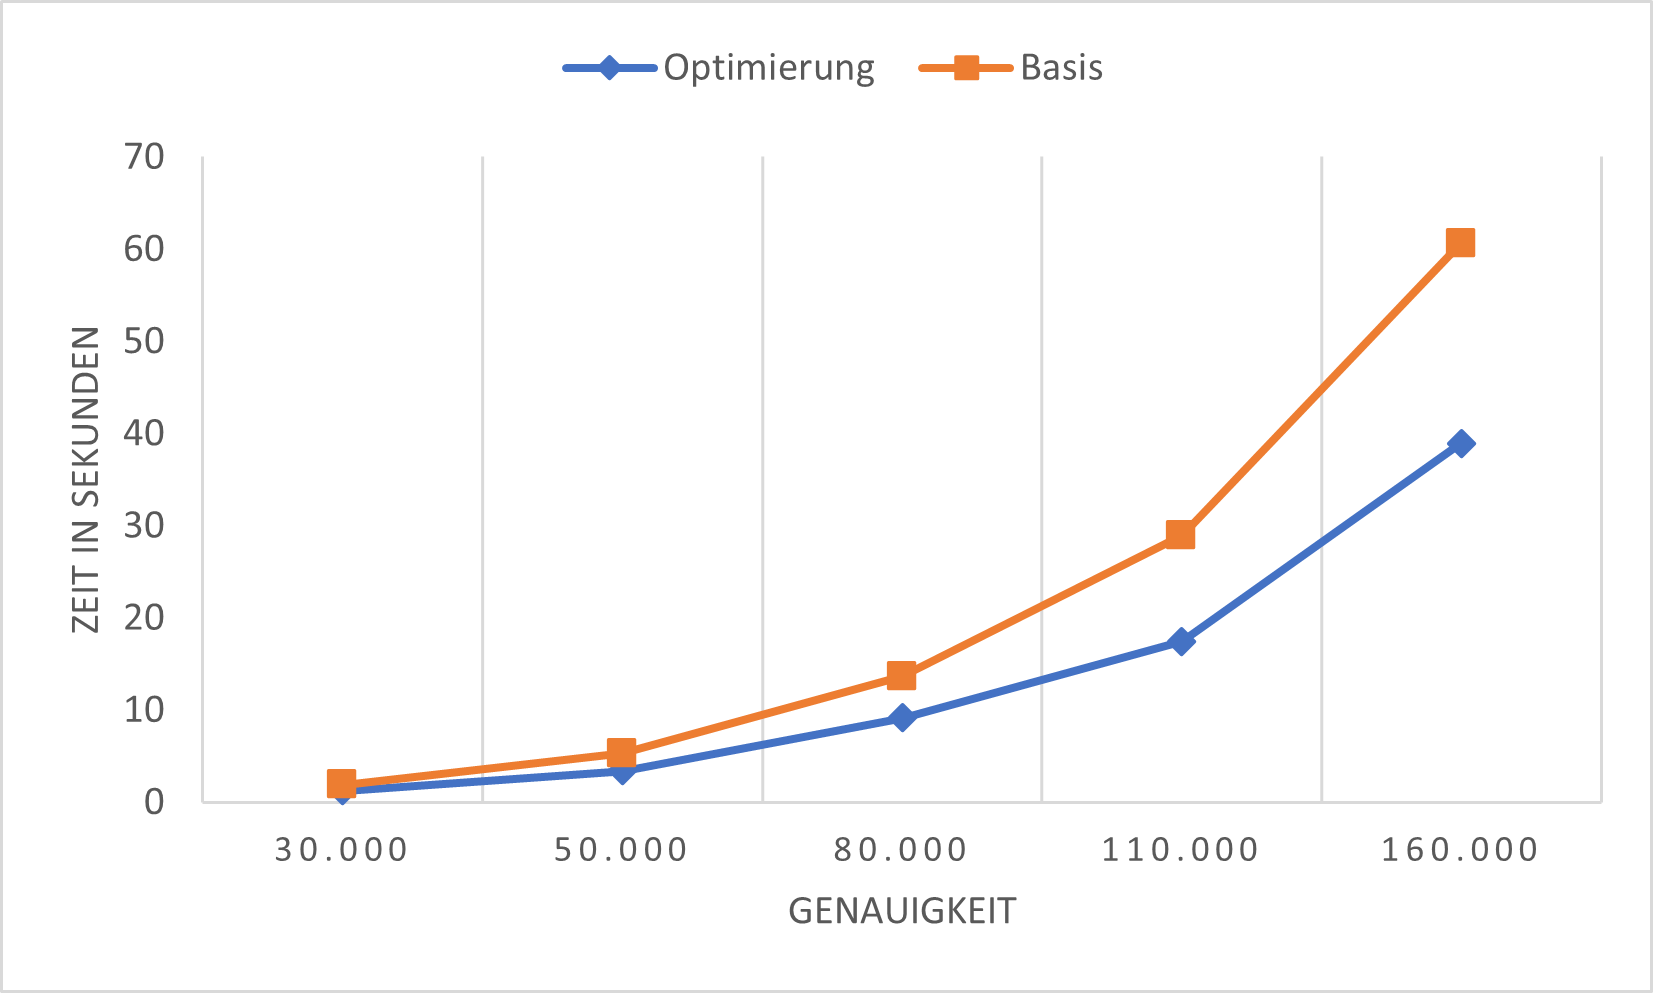
\includegraphics[scale = 1.0]{Images/PerformanceBig.png}
        \caption{Performancetest Big}
        \label{PerformanceBig}
    \end{figure}
    Die Abbildung 2 zeigt Eingaben von 1 bis 400 genauen Stellen.
    \begin{figure}
        \centering
        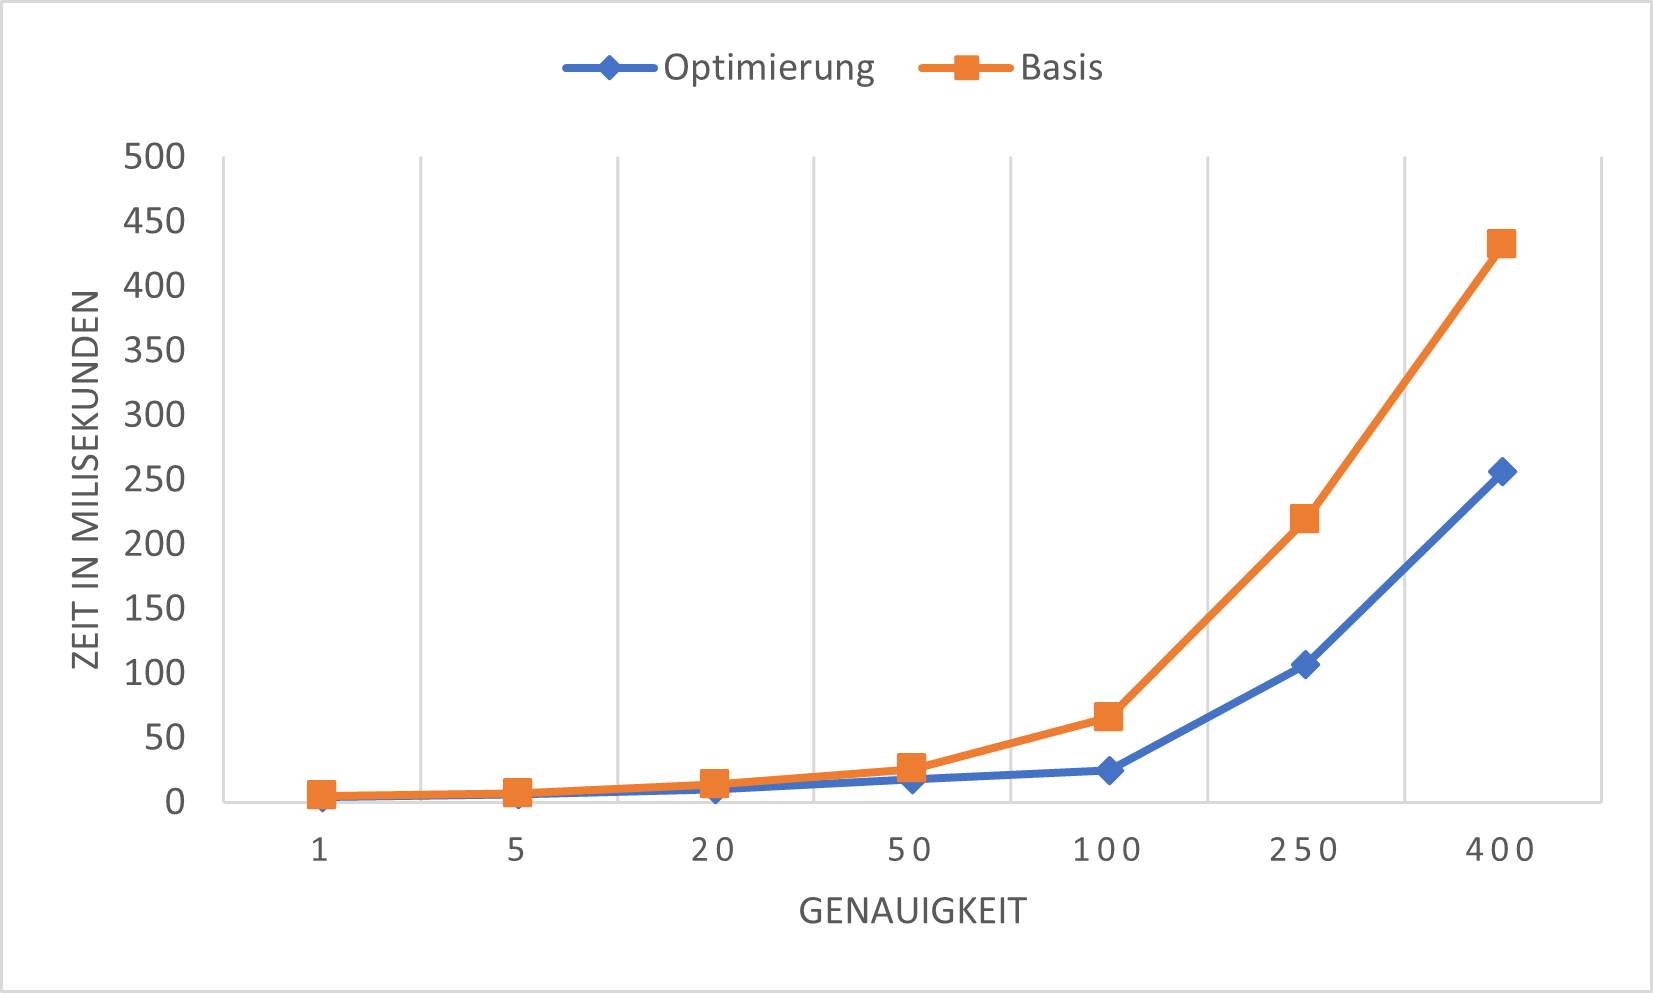
\includegraphics[scale = 1.0]{Images/PerformanceSmall.png}
        \caption{Performancetest Small}
        \label{PerformanceSmall}
    \end{figure}Die Performanceverbesserung ist deutlich in der Abflachung des Graphen zu sehen. Da in unserer Aufgabenstellung der schnellen Exponentiation ein hoher Wert zugesprochen wurde, vergleicht Abbildung 3 diese Methode, mit der Schleifen-Methode, in der die Matrix durch x-maliges Quadrieren berechnet wird. Es ergibt sich ein womöglich zuerst unerwartetes Bild ~\ref{FastExponentiationGraph}.
    \begin{figure}
        \centering
        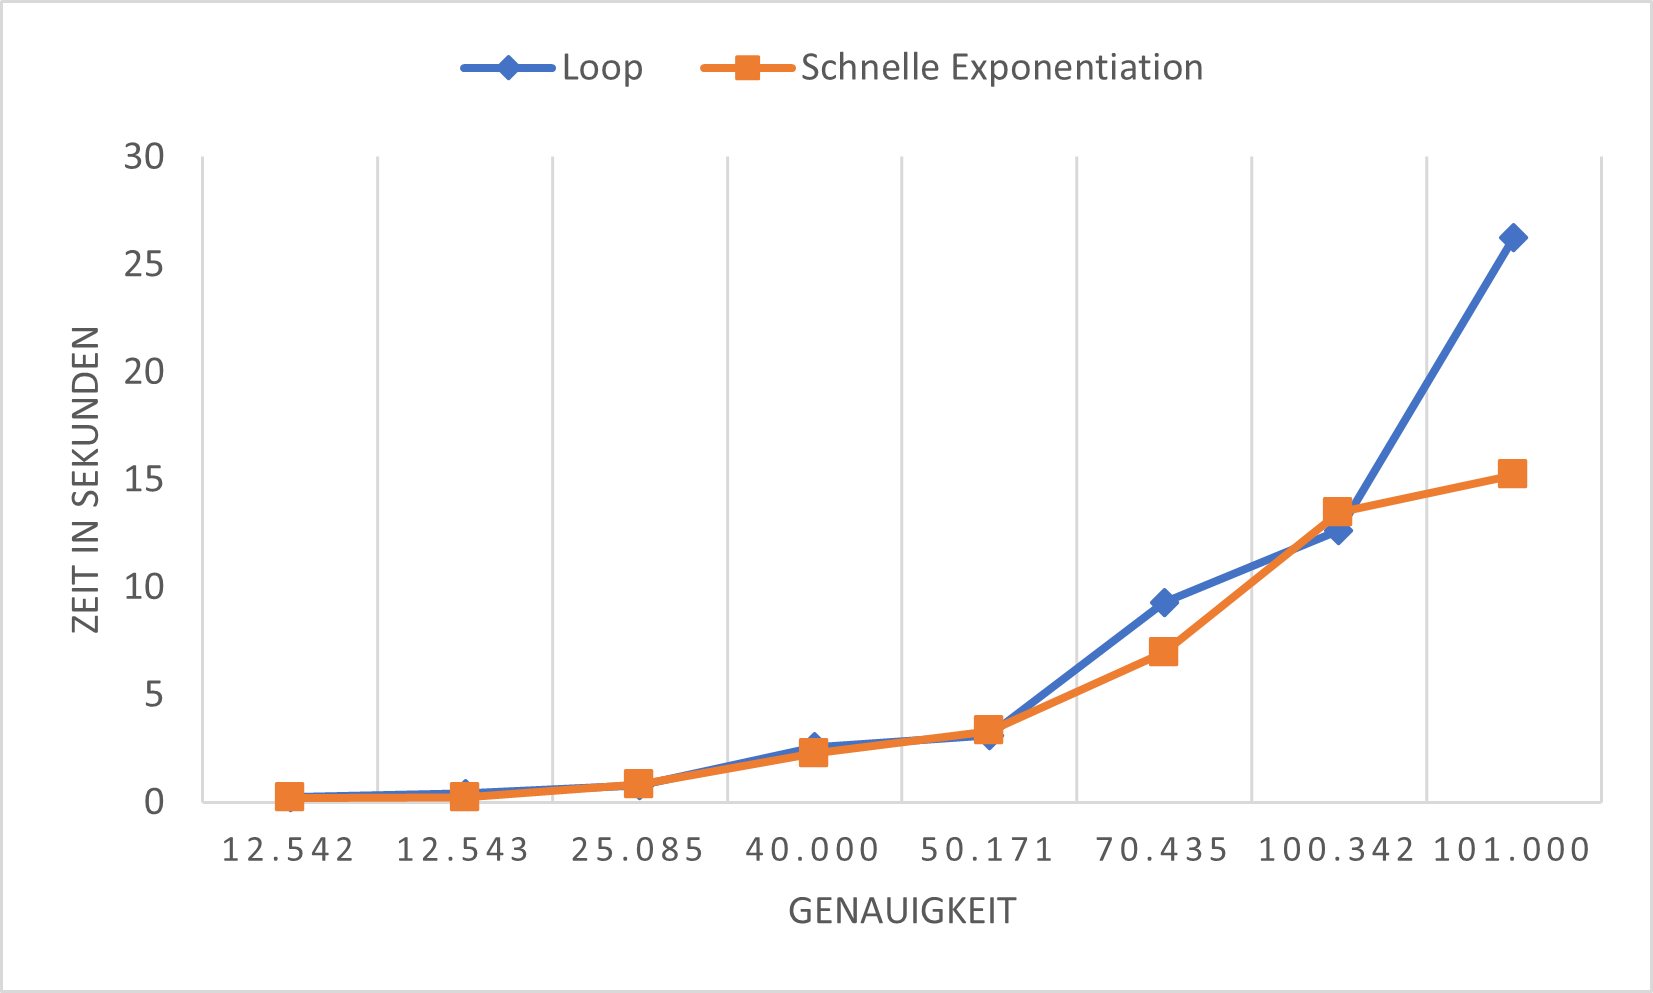
\includegraphics[scale = 1.0]{Images/Fast_NormalExponentiation.png}
        \caption{Vergleich: Schnelle Exponentiation}
        \label{FastExponentiationGraph}
    \end{figure}Die Werte erscheinen zuerst wohl willkürlich gewählt, doch die Werte 50.171, 100.342 sind genau die maximale Genauigkeit für 16 bzw. 17 Schleifendurchläufe. Wenn auch nur eine Stelle mehr benötigt wird, muss eine weitere Quadrierung der Matrix erfolgen, was exponentiell viel Zeit in Anspruch nimmt. So scheint es, dass die Schleife mit der schnellen Exponentiation anfangs gleichauf ist, jedoch sobald die Grenze für die Nachkommastellen, die mit einer bestimmten Anzahl an Schleifendurchläufen berechnet werden können, überschritten wird, ist die schnelle Exponentiation deutlich schneller (siehe 101.000). An der Grenze von 100.342 Stellen ist die Schleifen-Methode dem Algorithmus aber sogar überlegen. Da es für den Nutzer auch möglich sein soll, die Berechnung wahlweise in Hexadezimal ausgeben zu lassen, vergleicht Abbildung 4 \begin{figure}[ht]
                                                                                                                                                                                                                                                                                                                                                                                                                                                                                                                                                                                                                                                                                                                                                                                                                                                                                       \centering
                                                                                                                                                                                                                                                                                                                                                                                                                                                                                                                                                                                                                                                                                                                                                                                                                                                                                       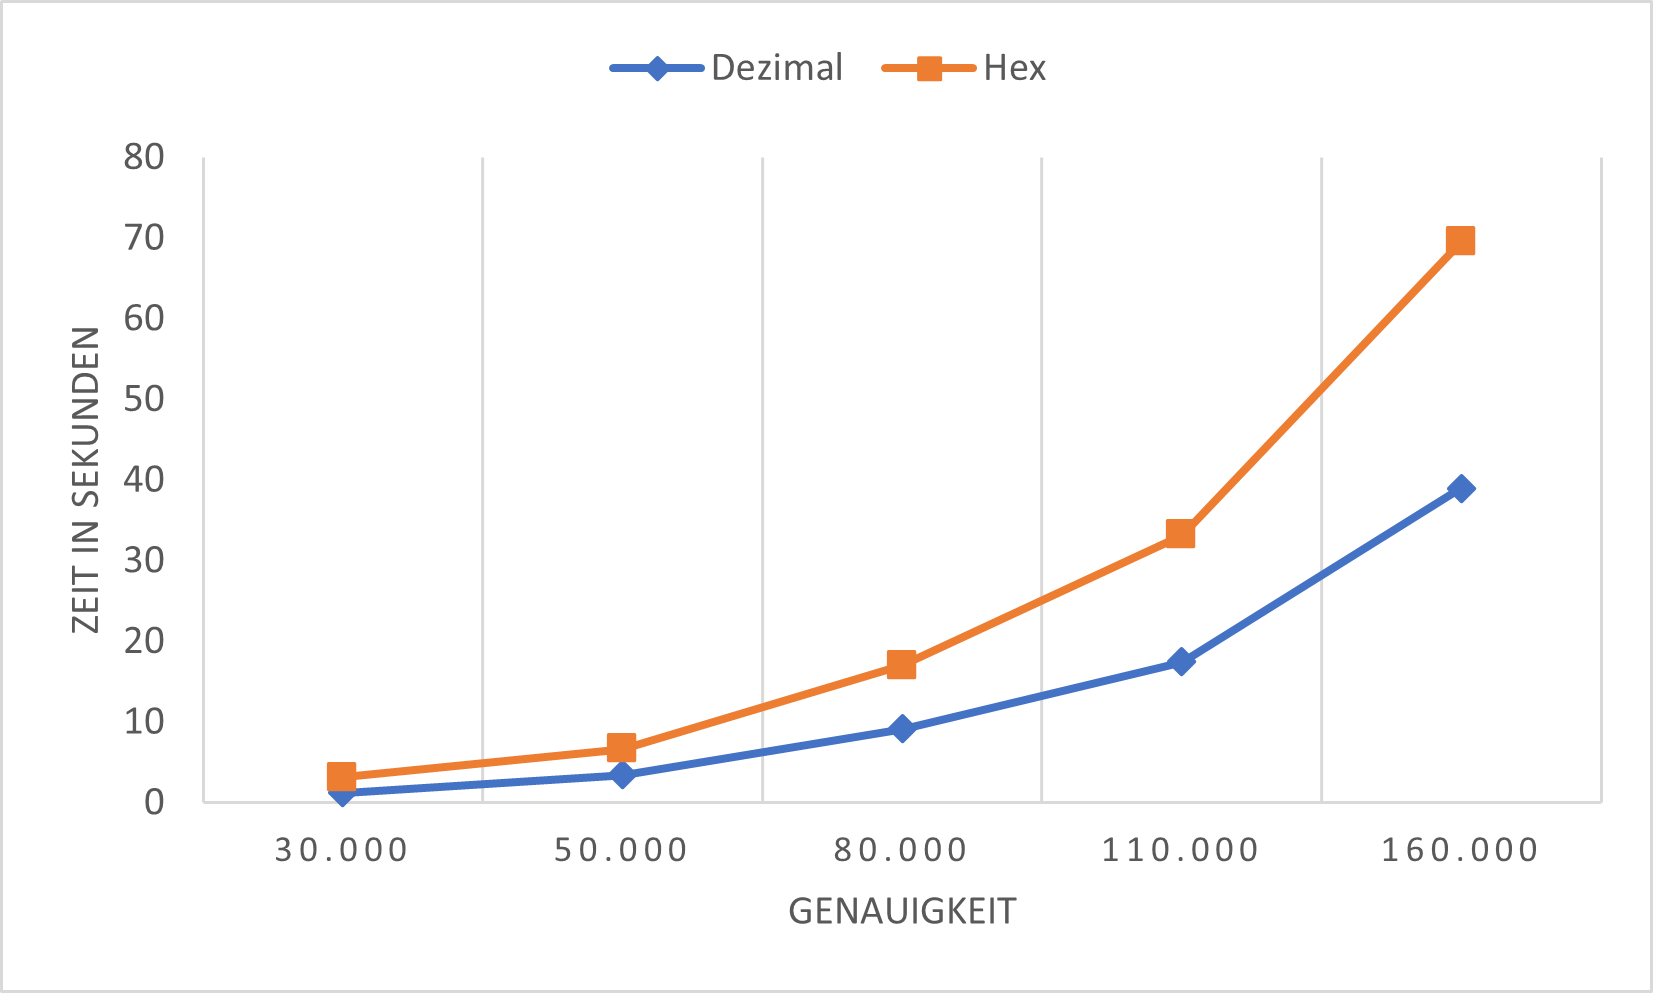
\includegraphics[scale = 1.0]{Images/HexDec.png}
                                                                                                                                                                                                                                                                                                                                                                                                                                                                                                                                                                                                                                                                                                                                                                                                                                                                                       \caption{Vergleih: Hex - Dec}
                                                                                                                                                                                                                                                                                                                                                                                                                                                                                                                                                                                                                                                                                                                                                                                                                                                                                       \label{HexDec}
    \end{figure} den Zeitunterschied, zwischen der Berechnung und der zusätzlichen Zeit, die benötigt wird, das Ergebnis in das Hexadezimal umzurechnen. (Die Zeit für die Berechnung ist in Hex auch enthalten). Dieser Vorgang könnte durch eine zweite Implementierung, die die Berechnungen mit Hexadezimalzahlen durchführt, optimiert werden, jedoch würde das den Rahmen dieses Projektes überschreiten und wurde deswegen nicht in den Code aufgenommen.
    \subsection{SIMD}
    SIMD wird in der Sub-Methode genutzt: Es werden gleichzeitig 4 Arrays des Subtrahenden von 4 des Minuenden abgezogen und in den Minuenden zurückgeschrieben, was eine merkbare Optimierung darstellt. Diese Verbesserung der Laufzeit war jedoch keine wirkliche Verbesserung, da der Compiler durch die 03 Flag SIMD schon von alleine genutzt hat, wodurch nach dieser Optimierung sich die Zeit in der Performanceanalyse nicht verändert hat.
    Eine Funktion, in der SIMD keinen Nutzen findet, ist die Divisionsmethode, da dort der Divisor solange vom Dividend abgezogen wird bis der Divisor größer als der Dividend ist. Und da nach jeder Subtraktion geprüft werden muss, welche Zahl nun größer ist, lassen sich die Subtraktionen nicht parallelisieren.
    \subsection{Int Arrays}
    Anfangs haben wir die Werte in Int Arrays gespeichert, in denen nur Zahlen zwischen 0 - 9999 stehen konnten, da größere Zahlen bei einer Multiplikation zu einem Overflow führen könnten. Gegenüber der Verwendung von Long-Arrays erwies sich diese Methode als deutlich ineffizienter, was sich dadurch erklären lässt, dass eine Zahl in weniger long Arrays aufgeteilt werden kann und somit weniger einzelne Arrays miteinander verrechnet werden. Aufgrund der bereits abgebildeten Performance-Diagramme verzichten wir aus Gründen der Übersichtlichkeit darauf, diesen speziellen Unterschied zusätzlich grafisch darzustellen.
    \section{Zusammenfassung und Ausblick}
    Unsere Aufgabe war es, mit Hilfe der schnellen Exponentiation ~\ref{Schnelle Exponentiation}, beliebig viele Nachkommastellen von $\sqrt{2}$ zu berechnen. Dazu mussten wir einen neuen Datentypen \glqq BigNum\grqq\space implementieren, der die gewünschte Anzahl an Stellen speichert. Die Schwierigkeit bestand darin, die Grundoperationen auf diesem Struct zu programmieren und dabei sicherzustellen, dass der benötigte Speicher auch immer verfügbar ist. Schnell ist klar geworden, dass die $2^{64}$ Nachkommastellen der Eingabe unrealistisch für den Rahmen dieses Projekts sind. Selbst im Internet findet man nicht auf Anhieb mehrere Millionen Stellen. Schlussendlich ist es uns gelungen eine funktionierende Implementierung bereitzustellen, diese weiter zu optimieren und mit Hilfe des Makefiles eine ausführbare Datei zu erstellen, die Inputs erwartet, die die gewünschte Ausgabe repräsentieren. Es stellt sich dennoch die Frage, welche Relevanz für derart viele Nachkommastellen besteht.

    \bibliographystyle{plain}
    \bibliography{Ausarbeitung}

\end{document}
